\section{Dimensionality Reduction: PCA}
\begin{frame}{The Curse of Dimensionality}

\textbf{Real-world data is high-dimensional:}

\vspace{0.8em}
\begin{columns}[c]
\begin{column}{0.48\textwidth}
\textbf{Examples:}
\begin{itemize}
\item Images: 1000$\times$1000 = 1M pixels
\item Text: 10,000+ words
\item Genomics: 20,000+ genes
\item Sensors: 100+ measurements
\end{itemize}

\vspace{1em}
\textbf{Problems:}
\begin{itemize}
\item Hard to visualize
\item Slow to compute
\item Lots of redundancy
\item Noisy measurements
\end{itemize}
\end{column}

\begin{column}{0.48\textwidth}
\centering
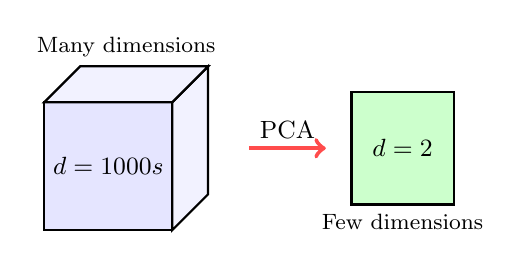
\begin{tikzpicture}[scale=0.65]
    % 3D cube representing high dimensions
    \draw[thick, fill=blue!10] (0,0) rectangle (2.5,2.5);
    \draw[thick, fill=blue!5] (2.5,0) -- (3.2,0.7) -- (3.2,3.2) -- (2.5,2.5) -- cycle;
    \draw[thick, fill=blue!5] (0,2.5) -- (0.7,3.2) -- (3.2,3.2) -- (2.5,2.5) -- cycle;
    
    \node at (1.25, 1.25) {\small $d = 1000s$};
    \node[above, font=\footnotesize] at (1.6, 3.2) {Many dimensions};
    
    % Arrow
    \draw[->, ultra thick, red!70] (4, 1.6) -- (5.5, 1.6);
    \node[above, font=\small] at (4.75, 1.6) {PCA};
    
    % 2D plane representing low dimensions
    \draw[thick, fill=green!20] (6,0.5) rectangle (8,2.7);
    \node at (7, 1.6) {\small $d = 2$};
    \node[below, font=\footnotesize] at (7, 0.5) {Few dimensions};
\end{tikzpicture}

\vspace{1em}
\textbf{Solution:}
Find a lower-dimensional representation while keeping important information (Dimensionality Reduction)
\end{column}
\end{columns}

\end{frame}

% --- SLIDE 2: What is PCA? ---
\begin{frame}{What is PCA?}

\textbf{Principal Component Analysis (PCA)} is a dimensionality reduction algorithm that finds the most important directions in your data.

\vspace{1em}
\begin{tcolorbox}[colback=blue!5, colframe=blue!50, title=\textbf{Core Idea}]
Instead of using original features, create \textbf{new features} (principal components) that:
\begin{itemize}
\item Capture maximum variance
\item Are uncorrelated with each other
\item Are ranked by importance
\end{itemize}

Then keep only the top few components!
\end{tcolorbox}

\vspace{1em}
\centering
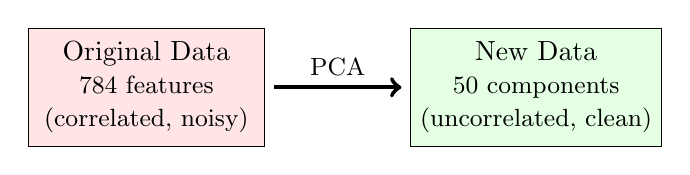
\begin{tikzpicture}[scale=0.9]
    \node[draw, rectangle, fill=red!10, minimum width=3cm, minimum height=1.5cm, align=center] at (0,0) {
        Original Data\\
        \small 784 features\\
        \small (correlated, noisy)
    };
    
    \draw[->, ultra thick] (1.8, 0) -- (3.6, 0) node[midway, above] {\small PCA};
    
    \node[draw, rectangle, fill=green!10, minimum width=3cm, minimum height=1.5cm, align=center] at (5.5,0) {
        New Data\\
        \small 50 components\\
        \small (uncorrelated, clean)
    };
\end{tikzpicture}

\end{frame}

% --- SLIDE 3: PCA Intuition - Finding Directions ---
\begin{frame}{PCA Intuition: Finding the Best Directions}

\textbf{Goal:} Find directions where data varies the most.

\vspace{0.5em}
\centering
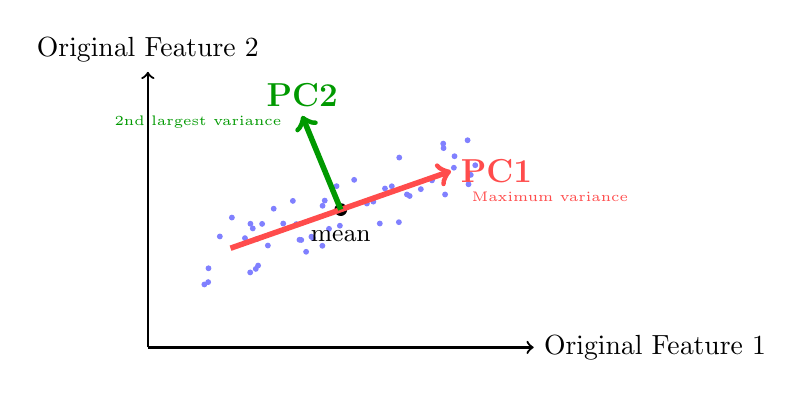
\begin{tikzpicture}[scale=0.7]
    % Data points (elongated cloud)
    \foreach \i in {1,...,50} {
        \pgfmathsetmacro{\x}{2.5*rand + 3.5}
        \pgfmathsetmacro{\y}{0.6*rand + 2.5 + 0.35*(\x-3.5)}
        \filldraw[blue!50] (\x, \y) circle (1.2pt);
    }
    
    % Mean point
    \filldraw[black] (3.5, 2.5) circle (3pt);
    \node[below] at (3.5, 2.3) {\small mean};
    
    % First principal component (main direction of variance)
    \draw[->, red!70, ultra thick, line width=2pt] (1.5, 1.8) -- (5.5, 3.2);
    \node[red!70, font=\large, right] at (5.5, 3.2) {\textbf{PC1}};
    \node[red!70, font=\tiny, below right] at (5.7, 3.0) {Maximum variance};
    
    % Second principal component (orthogonal)
    \draw[->, green!60!black, ultra thick, line width=2pt] (3.5, 2.5) -- (2.8, 4.2);
    \node[green!60!black, font=\large, above] at (2.8, 4.2) {\textbf{PC2}};
    \node[green!60!black, font=\tiny, above left] at (2.6, 3.8) {2nd largest variance};
    
    % Axes
    \draw[->, thick] (0, 0) -- (7, 0) node[right] {Original Feature 1};
    \draw[->, thick] (0, 0) -- (0, 5) node[above] {Original Feature 2};
\end{tikzpicture}

\vspace{0.8em}
\begin{itemize}
\item PC1: Direction with most spread
\item PC2: Perpendicular to PC1, next most spread
\item PC3, PC4, ... : Each perpendicular to all previous ones
\end{itemize}

\end{frame}

% --- SLIDE 4a: How Does PCA Work? (Part 1) ---
\begin{frame}{How Does PCA Work? (Part 1)}

\textbf{Step 1: Prepare the Data}

% \vspace{0.8em}
\begin{tcolorbox}[colback=gray!5, colframe=gray!80, title=\textbf{1. Center the Data}]
Shift the data so the center is at the origin (0,0).
% \vspace{0.5em}
\[
X_{\text{centered}} = X - \bar{X}
\]
\small \textit{(Subtract the mean from every feature)}
\end{tcolorbox}

% \vspace{1em}
\begin{tcolorbox}[colback=blue!5, colframe=blue!50, title=\textbf{2. Compute Covariance Matrix}]
Calculate how features vary with respect to each other.
\vspace{0.5em}
\[
C = \frac{1}{n} X_{\text{centered}}^\top X_{\text{centered}}
\]
\small \textit{(Finds correlations between features)}
\end{tcolorbox}

\end{frame}

% --- SLIDE 4b: How Does PCA Work? (Part 2) ---
\begin{frame}{How Does PCA Work? (Part 2)}

\textbf{Step 2: Find Directions \& Project}

% \vspace{0.8em}
\begin{tcolorbox}[colback=purple!5, colframe=purple!50, title=\textbf{3. Find Principal Components}]
Calculate \textbf{Eigenvectors} and \textbf{Eigenvalues} of the covariance matrix $C$.
\begin{itemize}
    \item \textbf{Eigenvectors:} The directions of the new axes.
    \item \textbf{Eigenvalues:} The amount of variance (information) along those axes.
\end{itemize}
\end{tcolorbox}

% \vspace{1em}
\begin{tcolorbox}[colback=red!5, colframe=red!50, title=\textbf{4. Select \& Project}]
Pick the top $k$ eigenvectors with the largest eigenvalues and transform the data.
\vspace{0.5em}
\[
Z = X_{\text{centered}} \cdot V_k
\]
\small \textit{(Reduces data from $d$ dimensions $\rightarrow$ $k$ dimensions)}
\end{tcolorbox}

\end{frame}

% --- SLIDE 6: Choosing Number of Components ---
\begin{frame}{How Many Components to Keep?}

\textbf{Key question:} How many components are enough?

\vspace{0.5em}
\centering
\textbf{Cumulative Variance Explained}

% \vspace{0.2em}
{\small (The most common method for selecting $K$)}

% \vspace{1em}
\centering
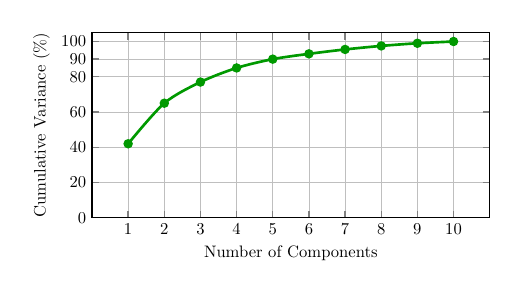
\begin{tikzpicture}[scale=0.6]
    \begin{axis}[
        width=10cm, height=5.5cm, % Made wider since it's alone now
        xlabel={Number of Components},
        ylabel={Cumulative Variance (\%)},
        grid=major,
        ymin=0, ymax=105,
        xmin=0, xmax=11,
        xtick={1,2,3,4,5,6,7,8,9,10},
        ytick={0,20,40,60,80,90,100},
        axis line style={thick},
        tick style={thick}
    ]
    % Cumulative Curve
    \addplot[green!60!black, ultra thick, mark=*, smooth] coordinates {
        (1,42) (2,65) (3,77) (4,85) (5,90) (6,93) (7,95.5) (8,97.5) (9,99) (10,100)
    };
    
    % % 90% Threshold Line
    % \draw[red, thick, dashed] (axis cs:0,90) -- (axis cs:11,90);
    % \node[red, font=\small, above] at (axis cs:2.5,90) {Target Threshold (e.g., 90\%)};
    
    % % Dropdown line showing K=5 hits the target
    % \draw[red, thick, dashed] (axis cs:5,0) -- (axis cs:5,90);
    % \node[red, font=\bfseries] at (axis cs:5.2, 85) {Select $K=5$};
    % \filldraw[red] (axis cs:5,90) circle (2.5pt);

    \end{axis}
\end{tikzpicture}

% \vspace{1em}
\begin{tcolorbox}[colback=blue!5, colframe=blue!50, width=0.9\linewidth]
\textbf{Rule of Thumb:} Choose the smallest $K$ that preserves \textbf{80--95\%} of the total variance.
\end{tcolorbox}

\end{frame}


% --- SLIDE 7a: MNIST Case Study (The Data) ---
\begin{frame}{Application 1: Data Visualization}

\textbf{The Data:} MNIST Digits, 70,000 handwritten digits (0--9).

\vspace{1em}
\begin{columns}[c]
\begin{column}{0.45\textwidth}
\textbf{The Challenge:}
\begin{itemize}
    \item Each image is $28 \times 28$ pixels.
    \item Total features: $28 \times 28 = \mathbf{784}$ dimensions!
    \item We cannot "see" in 784 dimensions.
\end{itemize}

\vspace{1em}
\textbf{Question:} Can we compress this to just \textbf{2D} to see how the digits relate?
\end{column}

\begin{column}{0.5\textwidth}
\centering
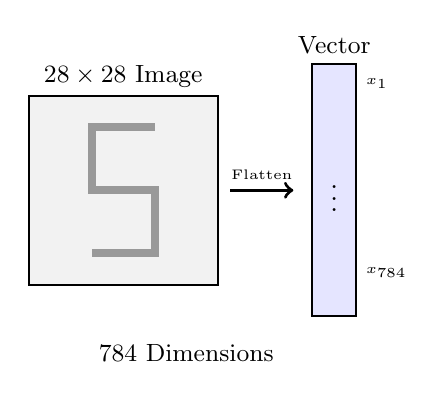
\begin{tikzpicture}[scale=0.8]
    % 2D Image Grid
    \draw[thick, fill=gray!10] (0,0) rectangle (3,3);
    \node at (1.5, 3.3) {\small $28 \times 28$ Image};
    
    % Draw a "Digit 5" roughly
    \draw[line width=3pt, gray!80] (2, 2.5) -- (1, 2.5) -- (1, 1.5) -- (2, 1.5) -- (2, 0.5) -- (1, 0.5);

    % Arrow
    \draw[->, very thick] (3.2, 1.5) -- (4.2, 1.5) node[midway, above, font=\tiny] {Flatten};

    % High-D Vector
    \draw[thick, fill=blue!10] (4.5, -0.5) rectangle (5.2, 3.5);
    \node at (4.85, 3.8) {\small Vector};
    \node at (4.85, 1.5) {\vdots};
    \node[right, font=\tiny] at (5.2, 3.2) {$x_1$};
    \node[right, font=\tiny] at (5.2, 0.2) {$x_{784}$};
    
    \node[below, align=center, font=\small] at (2.5, -0.8) {784 Dimensions};
\end{tikzpicture}
\end{column}
\end{columns}

\end{frame}

% --- SLIDE 7b: MNIST PCA Result ---
\begin{frame}[allowframebreaks]{Application 1: Data Visualization}

\textbf{Applying PCA:} We project the 784 dimensions down to the top 2 Principal Components.

\vspace{0.5em}
\centering

\begin{figure}
    \centering
    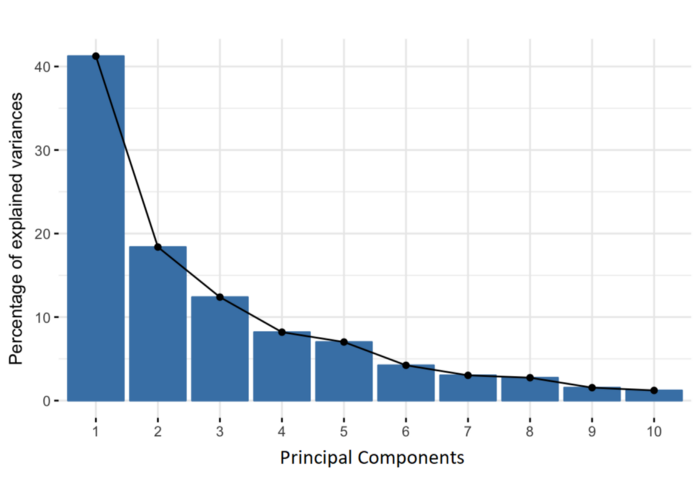
\includegraphics[width=0.8\linewidth]{images/PCA_Explained_VAR_MNIST.png}
    \label{fig:placeholder}
\end{figure}
\end{frame}

% --- SLIDE 7b: MNIST PCA Result ---
% --- SLIDE 7b: MNIST PCA Result & Critique ---
\begin{frame}{Application 1: Data Visualization}

\begin{columns}[c]
% --- LEFT COLUMN: Analysis ---
\begin{column}{0.45\textwidth}
    \textbf{Is this the best visualization?}
    
    \vspace{0.5em}
    \begin{itemize}
        \item It captures some structure, but points overlap heavily.
        \item \textbf{Reason:} PCA is \textbf{linear}, it cannot unfold complex, curved structures. 
        \item PCA is mostly used for compression. We will cover a better visualization algorithm shortly.
    \end{itemize}

\end{column}

% --- RIGHT COLUMN: Image ---
\begin{column}{0.55\textwidth}
    \centering
    % Ensure you have the file 'PCA_MNIST.png' in your project folder
    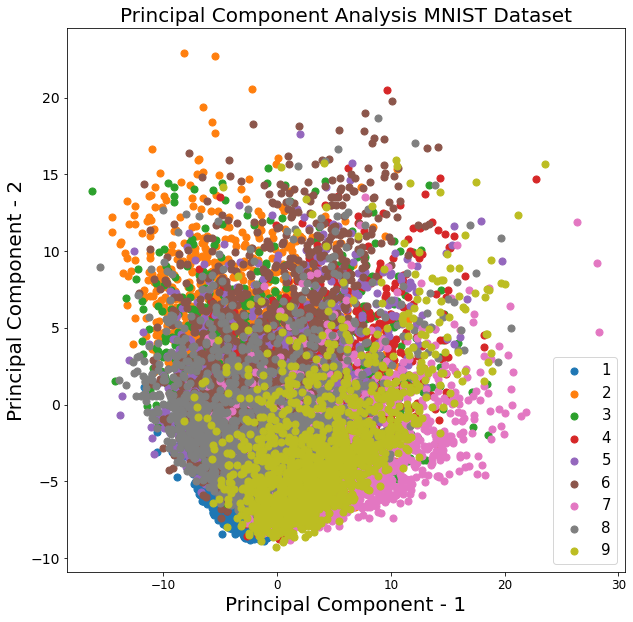
\includegraphics[width=\linewidth]{images/PCA_MNIST.png}
\end{column}
\end{columns}

\end{frame}
% --- SLIDE 8: Application 2 - Compression & Reconstruction ---
\begin{frame}{Application 2: Data Compression}

\textbf{Use case:} Store data more efficiently

\vspace{0.25em}
\centering
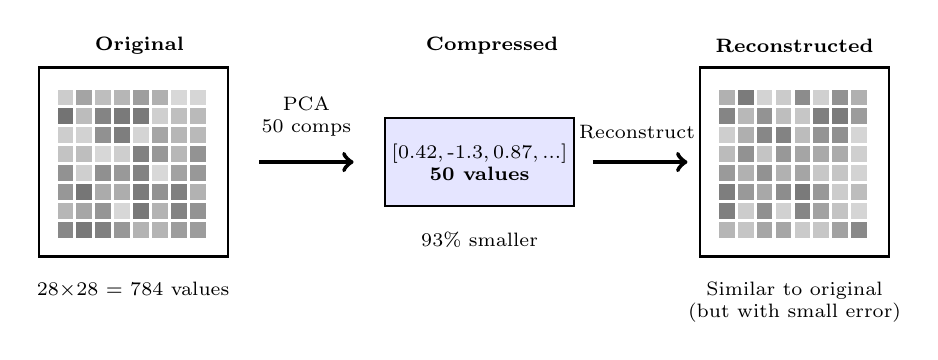
\begin{tikzpicture}[scale=0.80] % was 0.83
    % Original image
    \node[font=\scriptsize\bfseries] at (1.6, 3.35) {Original}; % slightly lower + smaller
    \draw[thick] (0,0) rectangle (3,3);
    \foreach \i in {0.3,0.6,...,2.7} {
        \foreach \j in {0.3,0.6,...,2.7} {
            \pgfmathsetmacro{\shade}{15 + 40*rnd}
            \fill[black!\shade] (\i,\j) rectangle +(0.25,0.25);
        }
    }
    \node[below, font=\scriptsize] at (1.5, -0.25) {28$\times$28 = 784 values}; % smaller

    % Arrow and compression info
    \draw[->, ultra thick] (3.5, 1.5) -- (5, 1.5);
    \node[above, font=\scriptsize, align=center] at (4.25, 1.75) {PCA\\50 comps}; % shorter text

    % Compressed representation
    \node[font=\scriptsize\bfseries] at (7.2, 3.35) {Compressed};
    \draw[thick, fill=blue!10] (5.5,0.8) rectangle (8.5,2.2);
    \node[align=center, font=\scriptsize] at (7, 1.5) {%
        [0.42,\,-1.3,\,0.87,\,...]\\
        \textbf{50 values}
    };
    \node[below, font=\scriptsize] at (7, 0.55) {93\% smaller};

    % Arrow back
    \draw[->, ultra thick] (8.8, 1.5) -- (10.3, 1.5);
    \node[above, font=\scriptsize] at (9.50, 1.72) {Reconstruct};

    % Reconstructed image
    \node[font=\scriptsize\bfseries] at (12, 3.35) {Reconstructed};
    \draw[thick] (10.5,0) rectangle (13.5,3);
    \foreach \i in {0.3,0.6,...,2.7} {
        \foreach \j in {0.3,0.6,...,2.7} {
            \pgfmathsetmacro{\shade}{15 + 38*rnd}
            \fill[black!\shade] (10.5+\i,\j) rectangle +(0.25,0.25);
        }
    }
    \node[below, font=\scriptsize, align=center] at (12, -0.25) {Similar to original\\(but with small error)};
\end{tikzpicture}

\vspace{0.15em}
\centering
\small \textbf{More components = better reconstruction, less compression}

\vspace{0.35em}
\begin{columns}[c]
\begin{column}{0.32\textwidth}
\centering
\small \textbf{10 PCs}\\99\% compression \\(blurry)
\end{column}
\begin{column}{0.32\textwidth}
\centering
\small \textbf{50 PCs}\\93\% compression \\(good)
\end{column}
\begin{column}{0.32\textwidth}
\centering
\small \textbf{200 PCs}\\75\% compression \\(near perfect)
\end{column}
\end{columns}

\end{frame}


% --- SLIDE 10: PCA Limitations ---
\begin{frame}{PCA Limitations}

\begin{columns}[c]
\begin{column}{1.0\textwidth}
\textbf{PCA Limitations:}

\begin{itemize}
\item \textbf{Linear only}: Finds linear combinations of features
\item \textbf{Sensitive to scale}: Must standardize data first
\item \textbf{Not Interpretable}: PCs are combinations of all features
\item \textbf{Outliers}: Can distort principal components
\end{itemize}

\end{column}
\end{columns}

\vspace{1em}
\centering
\small \textit{Let's have a look at a better algorithm for high dimensional data visualization...}

\end{frame}



% =========================
% t-SNE (Intuition Only)
% =========================

\section{Dimensionality Reduction: t-SNE}

% --- SLIDE: Why t-SNE? ---
